\documentclass[]{article}
\usepackage{lmodern}
\usepackage{amssymb,amsmath}
\usepackage{ifxetex,ifluatex}
\usepackage{fixltx2e} % provides \textsubscript
\ifnum 0\ifxetex 1\fi\ifluatex 1\fi=0 % if pdftex
  \usepackage[T1]{fontenc}
  \usepackage[utf8]{inputenc}
\else % if luatex or xelatex
  \ifxetex
    \usepackage{mathspec}
  \else
    \usepackage{fontspec}
  \fi
  \defaultfontfeatures{Ligatures=TeX,Scale=MatchLowercase}
\fi
% use upquote if available, for straight quotes in verbatim environments
\IfFileExists{upquote.sty}{\usepackage{upquote}}{}
% use microtype if available
\IfFileExists{microtype.sty}{%
\usepackage{microtype}
\UseMicrotypeSet[protrusion]{basicmath} % disable protrusion for tt fonts
}{}
\usepackage[margin=1in]{geometry}
\usepackage{hyperref}
\hypersetup{unicode=true,
            pdftitle={Tree size, exposure, and hydraulic traits interactively shape drought response in a temperate broadleaf forest},
            pdfauthor={Ian McGregor, Ryan Helcoski, Norbert Kunert, Alan Tepley, Valentine Herrmann, Joseph Zailaa, Atticus Stovall, Neil Pederson, Lawren Sack, Krista Anderson-Teixeira},
            pdfborder={0 0 0},
            breaklinks=true}
\urlstyle{same}  % don't use monospace font for urls
\usepackage{natbib}
\bibliographystyle{apalike}
\usepackage{color}
\usepackage{fancyvrb}
\newcommand{\VerbBar}{|}
\newcommand{\VERB}{\Verb[commandchars=\\\{\}]}
\DefineVerbatimEnvironment{Highlighting}{Verbatim}{commandchars=\\\{\}}
% Add ',fontsize=\small' for more characters per line
\usepackage{framed}
\definecolor{shadecolor}{RGB}{248,248,248}
\newenvironment{Shaded}{\begin{snugshade}}{\end{snugshade}}
\newcommand{\AlertTok}[1]{\textcolor[rgb]{0.94,0.16,0.16}{#1}}
\newcommand{\AnnotationTok}[1]{\textcolor[rgb]{0.56,0.35,0.01}{\textbf{\textit{#1}}}}
\newcommand{\AttributeTok}[1]{\textcolor[rgb]{0.77,0.63,0.00}{#1}}
\newcommand{\BaseNTok}[1]{\textcolor[rgb]{0.00,0.00,0.81}{#1}}
\newcommand{\BuiltInTok}[1]{#1}
\newcommand{\CharTok}[1]{\textcolor[rgb]{0.31,0.60,0.02}{#1}}
\newcommand{\CommentTok}[1]{\textcolor[rgb]{0.56,0.35,0.01}{\textit{#1}}}
\newcommand{\CommentVarTok}[1]{\textcolor[rgb]{0.56,0.35,0.01}{\textbf{\textit{#1}}}}
\newcommand{\ConstantTok}[1]{\textcolor[rgb]{0.00,0.00,0.00}{#1}}
\newcommand{\ControlFlowTok}[1]{\textcolor[rgb]{0.13,0.29,0.53}{\textbf{#1}}}
\newcommand{\DataTypeTok}[1]{\textcolor[rgb]{0.13,0.29,0.53}{#1}}
\newcommand{\DecValTok}[1]{\textcolor[rgb]{0.00,0.00,0.81}{#1}}
\newcommand{\DocumentationTok}[1]{\textcolor[rgb]{0.56,0.35,0.01}{\textbf{\textit{#1}}}}
\newcommand{\ErrorTok}[1]{\textcolor[rgb]{0.64,0.00,0.00}{\textbf{#1}}}
\newcommand{\ExtensionTok}[1]{#1}
\newcommand{\FloatTok}[1]{\textcolor[rgb]{0.00,0.00,0.81}{#1}}
\newcommand{\FunctionTok}[1]{\textcolor[rgb]{0.00,0.00,0.00}{#1}}
\newcommand{\ImportTok}[1]{#1}
\newcommand{\InformationTok}[1]{\textcolor[rgb]{0.56,0.35,0.01}{\textbf{\textit{#1}}}}
\newcommand{\KeywordTok}[1]{\textcolor[rgb]{0.13,0.29,0.53}{\textbf{#1}}}
\newcommand{\NormalTok}[1]{#1}
\newcommand{\OperatorTok}[1]{\textcolor[rgb]{0.81,0.36,0.00}{\textbf{#1}}}
\newcommand{\OtherTok}[1]{\textcolor[rgb]{0.56,0.35,0.01}{#1}}
\newcommand{\PreprocessorTok}[1]{\textcolor[rgb]{0.56,0.35,0.01}{\textit{#1}}}
\newcommand{\RegionMarkerTok}[1]{#1}
\newcommand{\SpecialCharTok}[1]{\textcolor[rgb]{0.00,0.00,0.00}{#1}}
\newcommand{\SpecialStringTok}[1]{\textcolor[rgb]{0.31,0.60,0.02}{#1}}
\newcommand{\StringTok}[1]{\textcolor[rgb]{0.31,0.60,0.02}{#1}}
\newcommand{\VariableTok}[1]{\textcolor[rgb]{0.00,0.00,0.00}{#1}}
\newcommand{\VerbatimStringTok}[1]{\textcolor[rgb]{0.31,0.60,0.02}{#1}}
\newcommand{\WarningTok}[1]{\textcolor[rgb]{0.56,0.35,0.01}{\textbf{\textit{#1}}}}
\usepackage{graphicx,grffile}
\makeatletter
\def\maxwidth{\ifdim\Gin@nat@width>\linewidth\linewidth\else\Gin@nat@width\fi}
\def\maxheight{\ifdim\Gin@nat@height>\textheight\textheight\else\Gin@nat@height\fi}
\makeatother
% Scale images if necessary, so that they will not overflow the page
% margins by default, and it is still possible to overwrite the defaults
% using explicit options in \includegraphics[width, height, ...]{}
\setkeys{Gin}{width=\maxwidth,height=\maxheight,keepaspectratio}
\IfFileExists{parskip.sty}{%
\usepackage{parskip}
}{% else
\setlength{\parindent}{0pt}
\setlength{\parskip}{6pt plus 2pt minus 1pt}
}
\setlength{\emergencystretch}{3em}  % prevent overfull lines
\providecommand{\tightlist}{%
  \setlength{\itemsep}{0pt}\setlength{\parskip}{0pt}}
\setcounter{secnumdepth}{0}
% Redefines (sub)paragraphs to behave more like sections
\ifx\paragraph\undefined\else
\let\oldparagraph\paragraph
\renewcommand{\paragraph}[1]{\oldparagraph{#1}\mbox{}}
\fi
\ifx\subparagraph\undefined\else
\let\oldsubparagraph\subparagraph
\renewcommand{\subparagraph}[1]{\oldsubparagraph{#1}\mbox{}}
\fi

%%% Use protect on footnotes to avoid problems with footnotes in titles
\let\rmarkdownfootnote\footnote%
\def\footnote{\protect\rmarkdownfootnote}

%%% Change title format to be more compact
\usepackage{titling}

% Create subtitle command for use in maketitle
\providecommand{\subtitle}[1]{
  \posttitle{
    \begin{center}\large#1\end{center}
    }
}

\setlength{\droptitle}{-2em}

  \title{Tree size, exposure, and hydraulic traits interactively shape drought
response in a temperate broadleaf forest}
    \pretitle{\vspace{\droptitle}\centering\huge}
  \posttitle{\par}
    \author{Ian McGregor, Ryan Helcoski, Norbert Kunert, Alan Tepley, Valentine
Herrmann, Joseph Zailaa, Atticus Stovall, Neil Pederson, Lawren Sack,
Krista Anderson-Teixeira}
    \preauthor{\centering\large\emph}
  \postauthor{\par}
    \date{}
    \predate{}\postdate{}
  
\usepackage{booktabs}
\usepackage{longtable}
\usepackage{array}
\usepackage{multirow}
\usepackage{wrapfig}
\usepackage{float}
\usepackage{colortbl}
\usepackage{pdflscape}
\usepackage{tabu}
\usepackage{threeparttable}
\usepackage{threeparttablex}
\usepackage[normalem]{ulem}
\usepackage{makecell}
\usepackage{xcolor}

\usepackage{float}
\usepackage{booktabs}
\usepackage{pdflscape}
\newcommand{\blandscape}{\begin{landscape}}
\newcommand{\elandscape}{\end{landscape}}
\usepackage{caption}
\captionsetup[table]{font=small}
\captionsetup[figure]{font=small}
\usepackage{dcolumn}

\begin{document}
\maketitle

\hypertarget{abstract}{%
\subsubsection{Abstract}\label{abstract}}

\emph{content from AGU abstract:} Here, we integrate forest census data
from a 25.6-ha ForestGEO plot in Virginia (USA), tree-ring records for
12 species representing \#\#\% of woody productivity, leaf hydraulic
trait measurements, and microhabitat data. Individual-level growth
responses to three droughts (1964-66, 1977, 1999) were stronger among
taller trees in dominant canopy positions, those in wetter microsites,
and for more drought-sensitive species as assessed by leaf traits
(turgor loss at less negative leaf water potential, greater shrinkage
with leaf dehydration), with substantial variation in the best predictor
variables across given droughts. We conclude that when droughts occur,
large dominant trees, drought sensitive species, and individuals in
moist microhabitats are likely to be most strongly affected.

\hypertarget{introduction}{%
\subsubsection{Introduction}\label{introduction}}

Understanding how and why trees respond to drought is critical to
predicting forest drought responses and climate change feedbacks.

Forests are diverse in terms of tree sizes and functional traits, and it
is known that trees varying in size and functional traits respond
differently to drought (e.g., \citep{bennett_larger_2015}; REFS).
Therefore, in order to understand whole-forest response to drought, we
need to know how responses vary by tree size/ species. To do so, there
are four fundamental questions that must be addressed:

\emph{First, how significant is the effect of individual drought years?}
Droughts are rarely explicitly defined in ecological studies
\citep{slette_how_2019}, yet no two droughts are the same. This study
addressed this by analyzing trees' resistance to drought within and
across three defined drought periods.

\emph{Second, what drives the observed tendency for large trees to
suffer more during drought?}\\
\citep{bennett_larger_2015} showed that in forests globally, large trees
suffer greater growth reductions during drought. However, this analysis
quantified tree size based on DBH, which has no direct mechanistic
meaning. This study proposed three major mechanisms (besides insects):
(1) inherently greater biophysical challenge of being tall; (2) greater
exposure of the crowns of large trees; and (3) greater water
availability. It is also expected that roots play a role, though these
hypotheses still need to be tested.

\emph{Third, how do species' traits influence drought response?}
Analyzing drought responses on the species level does not fully explain
mechanisms and is not feasible in diverse forests. The solution is a
trait-based approach. Leaf hydraulic traits hold more promise than more
commonly/traditionally-measured traits such as wood density and SLA
(Medeiros et al.).

\emph{Fourth, how do tree size and functional traits interact to
influence drought response?} It is possible that the pattern observed by
\citep{bennett_larger_2015} could be caused by smaller trees being more
drought resistant. Alternatively, larger trees may have more
drought-resistant traits as adpatations to greater biophysical
challenges.

\emph{Hypotheses}

\textbf{1. How significant are individual drought years on a long
time-frame trend?} 1.1 Individual drought scenario is a strong predictor
of drought stress.

\begin{verbatim}
* P1.1 - Drought stress is proportional to the severity of each drought.
\end{verbatim}

\textbf{2. Why do larger trees suffer greater growth declines during
drought?} Our forest displays the same trend as most forests globally
\citep{bennett_larger_2015}. (Note that Bennett et al.~2015 identified
only one study on tree growth responses to drought in the Eastern US
temperate deciduous biome. We know little about how tree size shapes
drought response in this biome.)

2.1 DBH is a strong predictor of drought stress.

\begin{verbatim}
* P2.2-Drought response increases with DBH at time of drought.
\end{verbatim}

2.2. Height is a strong predictor of drought stress.

\begin{verbatim}
* P2.2-Drought response increases with height at time of drought.
* P2.2a - Drought response is better predicted by height than DBH.
\end{verbatim}

2.3. Large trees suffer more during drought because of greater exposure
(to radiation, wind, etc.)--either in relation to neighboring trees or
because of position on landscape.

\begin{verbatim}
* P3.1- Trees currently in a dominant canopy position suffered more during drought. 
\end{verbatim}

2.4. Rooting volume/depth relative to water sources are critical in
drought response. Effects of drought on larger trees are mediated by the
fact that large trees have better access to water.

\begin{verbatim}
 * P3.2- drought response increases with topographic wetness index
\end{verbatim}

\textbf{3. Do species functional traits predict drought response?}

\begin{verbatim}
 * P3.1 - diffuse porous species are more sensitive than ring porous (previously observed in eastern dec forests- Elliot et al. 2015, Friedrichs et al. 2009)
 * P3.2 - higher percent leaf area predicts higher drought stress
 * P3.3 - higher leaf mass area correlates positively to drought resistance (more sclerophyllous vegetation [thick leaves] usually means more adaptation) [Abrams 1990] [Guerfel et al 2009]
 * P3.4 - TLP correlates negatively with drought resistance (NEVER tested),
 * P3.5 - higher wood density means more drought resistant
\end{verbatim}

\textbf{4. How are functional traits distributed across size classes,
and how does this affect size-resistance relationship?}

4.1. Larger/ more exposed trees have more drought resistant traits,
meaning size effects are buffered by traits\\
4.1\_alt. Larger trees suffer more because they have more drought
vulnerable traits.

\begin{verbatim}
 * P3.1a- TLP is lower (larger negative) in taller/canopy trees
 * P3.1b- diffuse porous species more common in understory 

 * P3.2- Inclusion of TLP / rp in model does not eliminate or significantly reduce effect of tree size.
\end{verbatim}

\textbf{I think for \#4 here the focus should be on hypotheses looking
at the overall trend compared to the specific scenarios?}

\textbf{4. How do droughts vary in their affect on tree resistance? }

\begin{verbatim}
* P4.1 - The combined-years scenario will have more explaining variables than the individual scenarios.
* P4.2 - Inclusion of leaf hydraulic traits does not eliminate or significantly reduce effect of tree size.
* P4.3 - Drought resistance for each scenario will be explained more by hydraulic traits than by the biophysical environment
\end{verbatim}

\hypertarget{methods}{%
\subsubsection{Methods}\label{methods}}

\emph{Study site} Research was conducted at the 25.6 ha ForestGEO
(Global Earth Observatory) study plot at the Smithsonian Conservation
Biology Institute (SCBI) in Virginia, USA (38°53'36.6``N, 78°
08'43.4''W) \citep{andersonteixeira_ctfs-forestgeo:_2015}. SCBI is
located in the central Appalachian Mountains at the northern edge of
Shenandoah National Park. Elevations range from 273-338m above sea level
\citep{gonzalezakre_patterns_2016} with a topographic relief of 65m
\citep{bourg_initial_2013}. Dominant species include \emph{Liriodendron
tulipifera}, oaks (\emph{Quercus} spp.), and hickories (\emph{Carya}
spp.).

\emph{Data collection and preparation} The SCBI ForestGEO plot was
censused in 2008, 2013, and 2018 following standard ForestGEO
protocols\ldots{} {[}DETAILS{]}. Here, we use \ldots(\emph{very brief
summary of which data we use for what purpose-- but some will be better
integrated with methods descriptions below})

We analyzed tree-ring data from the twelve species contributing most to
woody aboveground net primary productivity (ANPP\_stem) (Table 1), which
together comprised 97\% of whole-ecosystem ANPP\_stem between 2008 and
2013. Cores were collected in 2010-2011 or 2016-2017 from a breast
height of 1.3m using a 5mm increment borer. In 2010-2011, cores were
collected from randomly selected live trees were selected at random from
each species in 2010-2011, with at least 30 of those trees having a
diameter at breast height (DBH) of at least 10cm
\citep{bourg_initial_2013}. In 2016-2017, cores were collected from all
dead trees found in the annual mortality census
\citep{gonzalezakre_patterns_2016}. Cores were sanded, measured, and
cross-dated using standard procedures, as detailed in
\citep{helcoski_growing_2019}. The resulting chronologies have been
published in association with \citep{helcoski_growing_2019}: (GitHub
URL), (ITRDB).

Height measurements (n=\# trees) were taken by several researchers
between 2012 to 2019, and are archived in a public GitHub repository
(\emph{GitHUB URL}). Measurement methods included manual
\citep[NEON]{stovall_assessing_2018}, digital rangefinders
\citep{andersonteixeira_size-related_2015}, and automatic LiDAR
\citep{stovall_terrestrial_2018}. Rangefinders either used the tangent
method (Impulse 200LR, TruPulse 360R) or the sine method (Nikon
ForestryPro) for calculating heights. The associated errors for using
either method were acknowledged \citep{larjavaara_measuring_2013}.
Species-specific height allometries were developed (Table S\# -
\textbf{ADD THIS TABLE TO SI}). For species that didn't have enough
height measurements, heights were calculated from equations derived from
all species in the study.

For each tree, we combined tree-ring records and allometric equations of
height and bark thickness to retroactively calculate DBH and estimate
height for the years 1950-2009. Prior DBH was estimated using the
following equation, using 2008 as the earliest year for having reliable
DBH measurements:

\[ diamYEAR = dbh2008 - 2*(bark.depth2008) - 2*\Sigma(ring.widthYEAR:ring.width2008) + 2*(bark.depth_YEAR) \]

Here, \emph{ring.width} was measured from cores. Bark thickness was
estimated from species-specific allometries based on the bark thickness
data of \citep{andersonteixeira_size-related_2015}. Specifically, we
used linear regression equations on log-transformed data to relate bark
thickness to DBH (Table S\#- \textbf{create table to give these
equations in SI}) and then used these to estimate bark thickness based
on DBH.

Crown positions were recorded in the field during the growing season of
2018 following the crown position protocol from
\citep{jennings_assessing_1999}, whereby positions were ranked as
dominant, codominant, intermediate, or suppressed. As there was no way
to retroactively estimate crown position, we assumed that 2018 crown
position was reflective of each tree's position over the past 60 years.
While some trees undoubtedly changed position, an analysis of crown
position relative to height (Fig. XX) and height change since
\emph{1959} indicated that change was likely slow. {[}\textbf{work on
this-- provide details?}{]}

Topographic wetness index (TWI) was calculated using the
\citep{R-dynatopmodel} package in R.

Hydraulic traits were collected from SCBI and are summarized in Table 1.
In August 2018, we collected leaf samples from three individuals of each
species \ldots{} (\textbf{Nobby's description of methods for the
following}) 1. PLA 2. LMA 4. Wood density 5. TLP

\textbf{Table 1. Species analyzed here, listed in descending order of
ANPP\_stem. n cores and DBH range represented, and species traits}
{[}*This replaces/combines the two remaining tables in this section.
Suggested columns, with those to include only if they fit in
parentheses: species, (stems \textgreater=10 cm per ha in plot),
(ANPP\_stem), n cores, DBH range of cores, (n cores in each crown
position) species means for each trait{]}

\begin{table}[H]
\centering
\begin{tabular}{l|r|r|r|r|r|r}
\hline
sp & n\_cores & dominant & co-dominant & intermediate & suppressed & prior dead\\
\hline
caco & 13 & NA & 2 & 5 & 5 & 1\\
\hline
cagl & 31 & 1 & 8 & 16 & 5 & 1\\
\hline
caovl & 23 & 4 & 5 & 12 & 2 & NA\\
\hline
cato & 13 & NA & NA & 6 & 2 & 5\\
\hline
fagr & 80 & NA & 7 & 48 & 25 & NA\\
\hline
fram & 62 & NA & 17 & 19 & 14 & 12\\
\hline
juni & 31 & NA & 21 & 8 & NA & 2\\
\hline
litu & 98 & 9 & 29 & 25 & 30 & 5\\
\hline
qual & 61 & 4 & 34 & 20 & 3 & NA\\
\hline
qupr & 59 & 1 & 26 & 20 & 12 & NA\\
\hline
quru & 69 & 6 & 36 & 23 & 2 & 2\\
\hline
quve & 77 & 6 & 46 & 22 & 1 & 2\\
\hline
\end{tabular}
\end{table}
\begin{table}[H]
\centering
\begin{tabular}{l|l|r|r|r}
\hline
Trait & Unit & mean & min & max\\
\hline
Ring Porosity & ring, semi-ring, diffuse & NA & NA & NA\\
\hline
Percent Leaf Area & \% & 15.09 & 8.52 & 24.64\\
\hline
Leaf Mass Area & g/m2 & 53.50 & 30.68 & 75.80\\
\hline
Wood density & g/cm3 & 0.70 & 0.40 & 1.09\\
\hline
TLP & MPa & -2.36 & -2.76 & -1.92\\
\hline
\end{tabular}
\end{table}

\emph{Climate and drought years} {[}\textbf{add description of climate
data used in Fig. 1, NEON vertical profiles}{]}

To accurately understand climate sensitivity, this study used a specific
definition of drought, which is not a common practice
\citep{slette_how_2019}. We used the pointRes package \citep{R-pointRes}
in R (version 3.5.3) to determine drought periods based on trees'
drought resistance, which is defined by \citep{lloret_components_2011}
as the ratio between the performance during and before the disturbance.
Candidate drought years were defined if \textgreater50\% of the cored
trees experienced \textless30\% growth in a year compared to the
previous 5 years. These were then cross-validated with the regional
Palmer Drought Severity Index (PDSI) values for each year, which yielded
a set of three periods that were consistently shown as drought:
1964-1966, 1977, and 1999.

\textbf{Figure 1. Time series of peak growing season (May-August)
climate conditions and residual chronologies for each species.} Droughts
analyzed here are indicated by dashed lines, and shading indicates the
pre-drought period used in calculations of the resistance metric. Figure
modified from \citep{helcoski_growing_2019}.
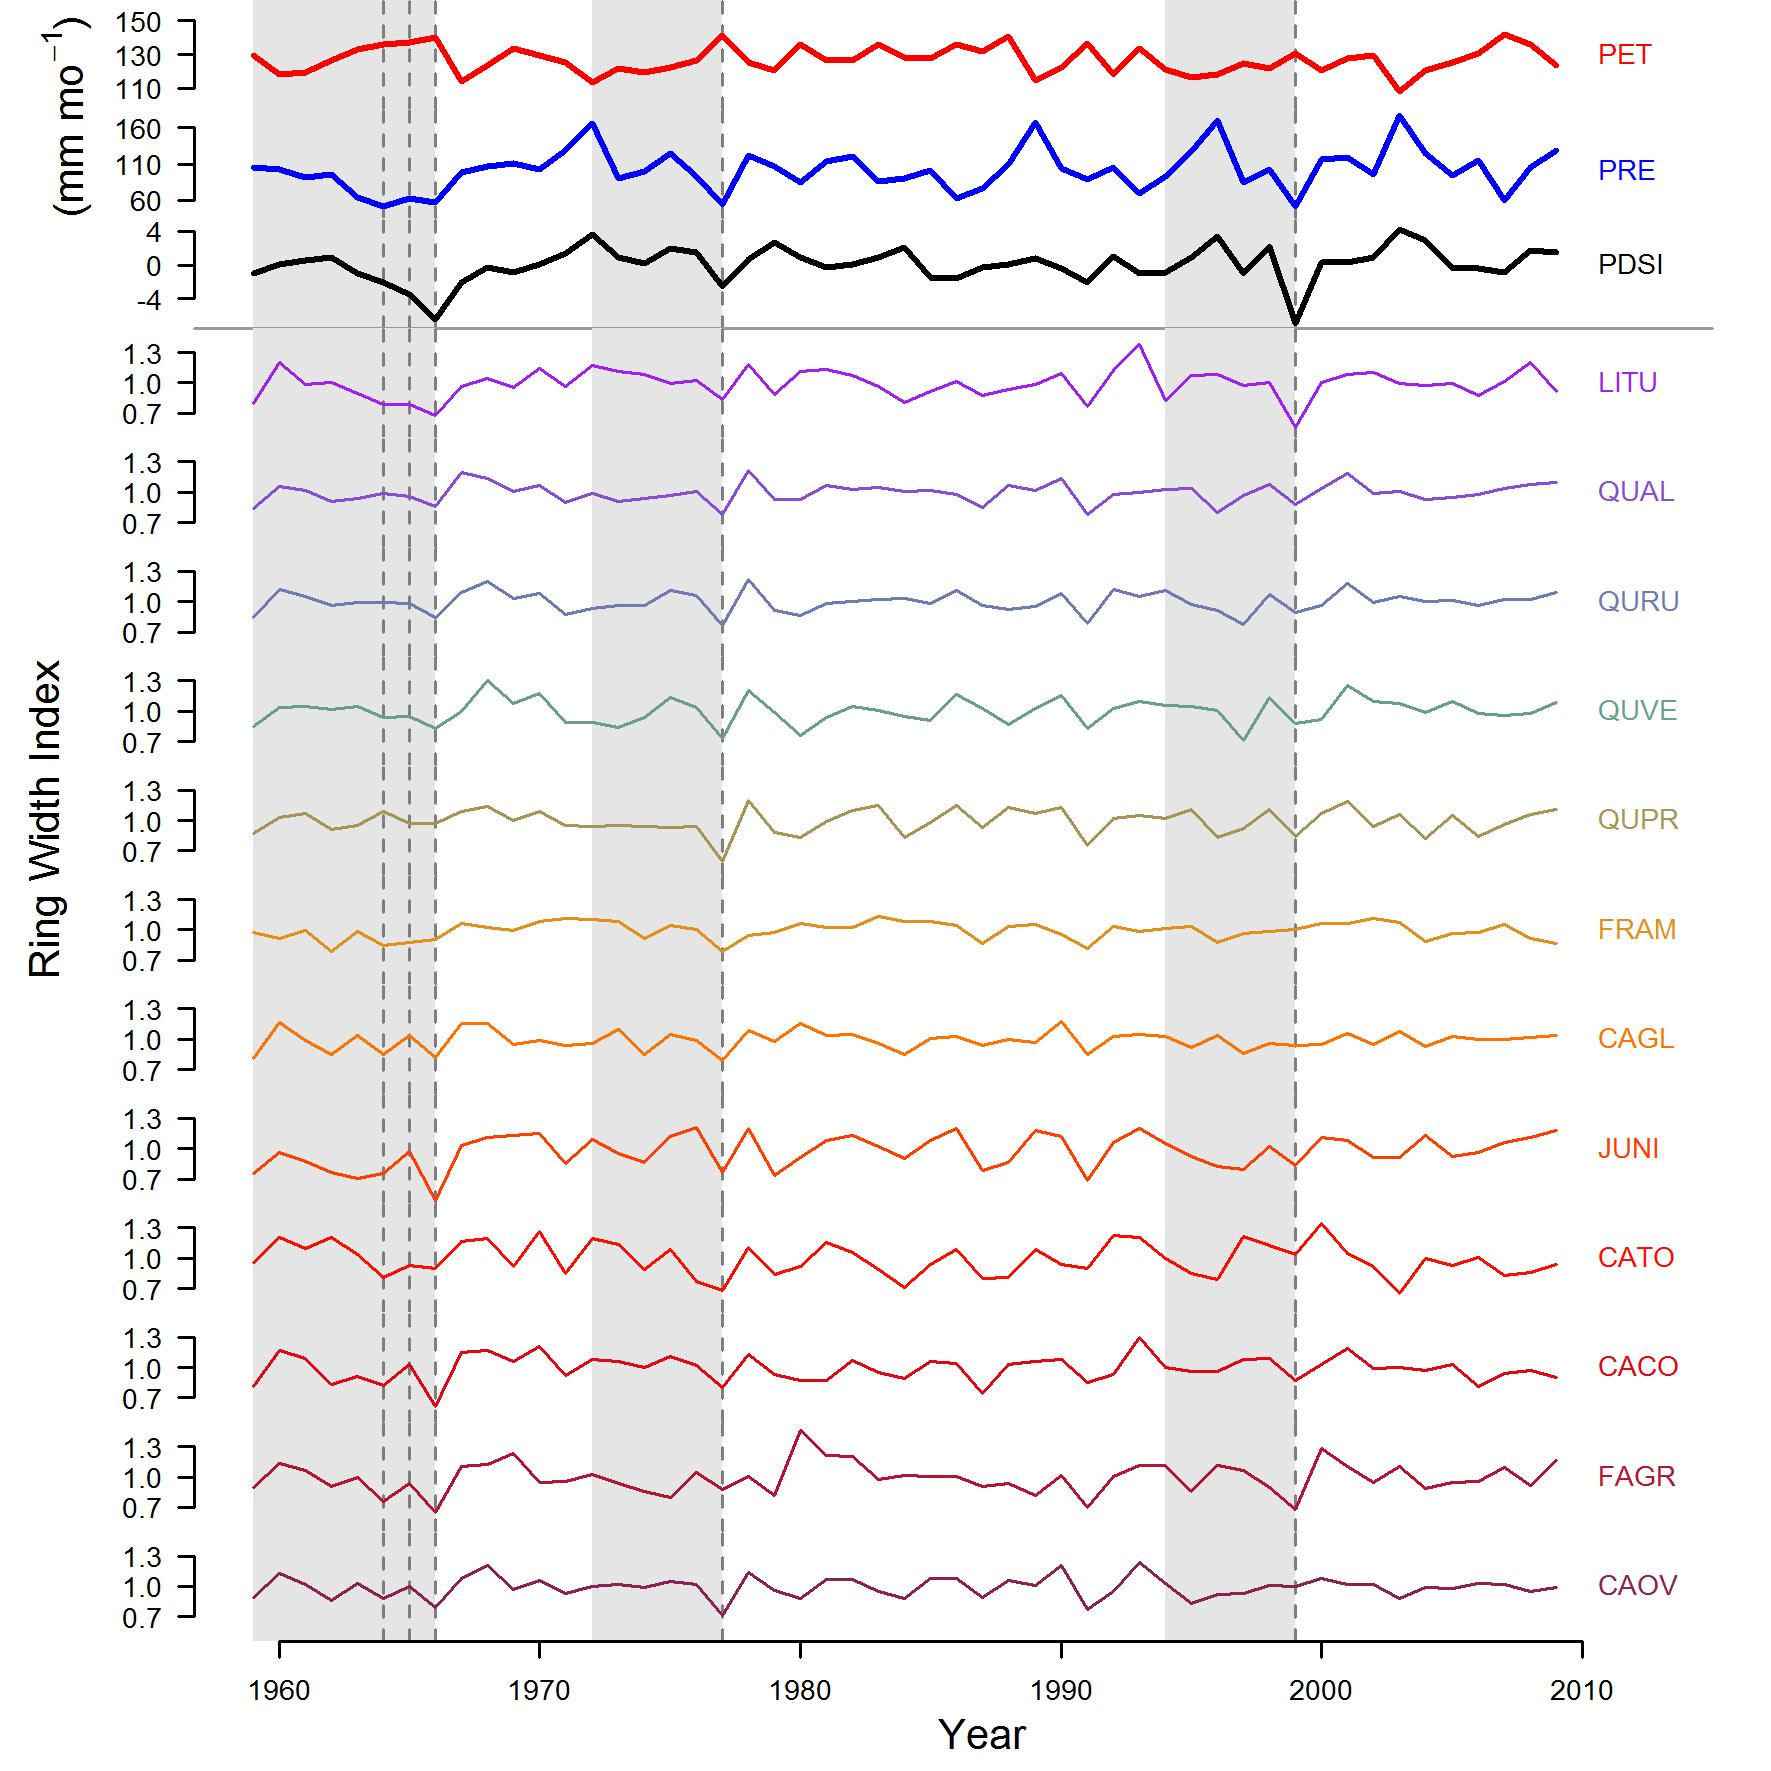
\includegraphics[width=5.20833in,height=\textheight]{tables_figures/Time_series_for_each_species.jpg}

\hypertarget{results}{%
\subsubsection{Results}\label{results}}

Once the data was collected, linear mixed models were run following the
order of the hypotheses as seen in Figure ???
{[}individual\_tested\_traits{]}. Using the \citep{R-pointRes} package,
we set up models with the resistance value as the response variable, and
each prediction's variable as the independent variable. Variables'
importance in predicting drought tolerance was calculated from
mixed-effects models and the lowest AICc
\citep[\citet{R-AICcmodavg}]{R-lme4}.Null models were determined in
order of the predictions. First, we analyzed the combined scenario to
determine if ``year'' was significant. Upon establishing this, we tested
height and DBH as size parameters. Although both were significant,
height was kept due to its larger delta AICc compared with the null
model. We then tested the remaining biophysical and hydraulic traits
individually against a null model containing height and year. This
yielded Figure ??? (cand\_full). All variables with dAICc \textgreater2
were used as candidates for each scenario's best model (figure ????
(tested\_traits\_best))

\begin{landscape}\begin{table}[t]

\caption{\label{tab:Table 1}All variables tested for climate sensitivity against appropriate null models, in line with hypothesis predictions. Each variable was tested for each drought scenario excepting "year" }
\centering
\begin{tabular}{rllllllrllrllrllrll}
\toprule
prediction & variable & variable\_description & null\_model & tested\_model & null\_model\_year & tested\_model\_year & dAIC\_all & coef\_all & coef\_var\_all & dAIC\_1964.1966 & coef\_1964.1966 & coef\_var\_1964.1966 & dAIC\_1977 & coef\_1977 & coef\_var\_1977 & dAIC\_1999 & coef\_1999 & coef\_var\_1999\\
\midrule
1.1 & year & drought.year & resist.value \textasciitilde{} (1|sp/tree) & resist.value \textasciitilde{} (1|sp/tree)+year & resist.value \textasciitilde{} (1|sp) & resist.value \textasciitilde{} (1|sp) & 35.834 & - & year1977 (-0.09), year1999 (-0.081) & 0.000 & NA & NA & 0.000 & NA & NA & 0.000 & NA & NA\\
2.1 & dbh.ln.cm & ln[DBH] & resist.value \textasciitilde{} year+(1|sp/tree) & resist.value \textasciitilde{} year+(1|sp/tree)+dbh.ln.cm & resist.value \textasciitilde{} (1|sp) & resist.value \textasciitilde{} (1|sp)+dbh.ln.cm & 7.411 & - & dbh.ln.cm (-0.035) & 18.276 & - & dbh.ln.cm (-0.082) & -0.947 & - & dbh.ln.cm (-0.021) & -1.918 & + & dbh.ln.cm (0.006)\\
2.2 & height.ln.m & ln[height] & resist.value \textasciitilde{} year+(1|sp/tree) & resist.value \textasciitilde{} year+(1|sp/tree)+height.ln.m & resist.value \textasciitilde{} (1|sp) & resist.value \textasciitilde{} (1|sp)+height.ln.m & 7.591 & - & height.ln.m (-0.058) & 17.788 & - & height.ln.m (-0.133) & -1.077 & - & height.ln.m (-0.032) & -2.022 & + & height.ln.m (0.002)\\
3.3 & position\_all & crown.position & resist.value \textasciitilde{} height.ln.m+year+(1|sp/tree) & resist.value \textasciitilde{} height.ln.m+year+(1|sp/tree)+position\_all & resist.value \textasciitilde{} height.ln.m+(1|sp) & resist.value \textasciitilde{} height.ln.m+(1|sp)+position\_all & 1.682 & - & position\_alldominant (-0.044), position\_allintermediate (-0.042), position\_allsuppressed (-0.053) & -2.548 & - & position\_alldominant (-0.055), position\_allintermediate (0.007), position\_allsuppressed (-0.044) & -0.700 & - & position\_alldominant (-0.076), position\_allintermediate (-0.033), position\_allsuppressed (0.029) & 4.087 & - & position\_alldominant (-0.003), position\_allintermediate (-0.082), position\_allsuppressed (-0.102)\\
3.4 & TWI & topographic.wetness.index & resist.value \textasciitilde{} height.ln.m+year+(1|sp/tree) & resist.value \textasciitilde{} height.ln.m+year+(1|sp/tree)+TWI & resist.value \textasciitilde{} height.ln.m+(1|sp) & resist.value \textasciitilde{} height.ln.m+(1|sp)+TWI & 2.631 & - & TWI (-0.009) & -0.563 & + & TWI (0.009) & 5.264 & - & TWI (-0.02) & 3.037 & - & TWI (-0.015)\\
\addlinespace
4.1 & rp & ring.porosity & resist.value \textasciitilde{} height.ln.m+year+(1|sp/tree) & resist.value \textasciitilde{} height.ln.m+year+(1|sp/tree)+rp & resist.value \textasciitilde{} height.ln.m+(1|sp) & resist.value \textasciitilde{} height.ln.m+(1|sp)+rp & -3.553 & + & rpring (0.04), rpsemi-ring (0.013) & -2.161 & + & rpring (0.101), rpsemi-ring (0.015) & 0.895 & - & rpring (-0.19), rpsemi-ring (-0.147) & 4.083 & + & rpring (0.2), rpsemi-ring (0.151)\\
4.2 & PLA\_dry\_percent & percent.leaf.area & resist.value \textasciitilde{} height.ln.m+year+(1|sp/tree) & resist.value \textasciitilde{} height.ln.m+year+(1|sp/tree)+PLA\_dry\_percent & resist.value \textasciitilde{} height.ln.m+(1|sp) & resist.value \textasciitilde{} height.ln.m+(1|sp)+PLA\_dry\_percent & 4.413 & - & PLA\_dry\_percent (-0.011) & 5.825 & - & PLA\_dry\_percent (-0.016) & -0.190 & - & PLA\_dry\_percent (-0.01) & -0.701 & - & PLA\_dry\_percent (-0.007)\\
4.3 & LMA\_g\_per\_m2 & leaf.mass.area & resist.value \textasciitilde{} height.ln.m+year+(1|sp/tree) & resist.value \textasciitilde{} height.ln.m+year+(1|sp/tree)+LMA\_g\_per\_m2 & resist.value \textasciitilde{} height.ln.m+(1|sp) & resist.value \textasciitilde{} height.ln.m+(1|sp)+LMA\_g\_per\_m2 & -1.895 & + & LMA\_g\_per\_m2 (0.001) & -1.075 & + & LMA\_g\_per\_m2 (0.002) & -1.698 & - & LMA\_g\_per\_m2 (-0.001) & -1.985 & + & LMA\_g\_per\_m2 (0)\\
4.4 & mean\_TLP\_Mpa & mean.turgor.loss.point & resist.value \textasciitilde{} height.ln.m+year+(1|sp/tree) & resist.value \textasciitilde{} height.ln.m+year+(1|sp/tree)+mean\_TLP\_Mpa & resist.value \textasciitilde{} height.ln.m+(1|sp) & resist.value \textasciitilde{} height.ln.m+(1|sp)+mean\_TLP\_Mpa & 4.580 & - & mean\_TLP\_Mpa (-0.207) & 1.352 & - & mean\_TLP\_Mpa (-0.217) & 1.008 & - & mean\_TLP\_Mpa (-0.236) & 0.132 & - & mean\_TLP\_Mpa (-0.177)\\
4.5 & WD\_g\_per\_cm3 & wood.density & resist.value \textasciitilde{} height.ln.m+year+(1|sp/tree) & resist.value \textasciitilde{} height.ln.m+year+(1|sp/tree)+WD\_g\_per\_cm3 & resist.value \textasciitilde{} height.ln.m+(1|sp) & resist.value \textasciitilde{} height.ln.m+(1|sp)+WD\_g\_per\_cm3 & -2.018 & + & WD\_g\_per\_cm3 (0.005) & -1.960 & - & WD\_g\_per\_cm3 (-0.049) & -1.236 & - & WD\_g\_per\_cm3 (-0.175) & 0.171 & + & WD\_g\_per\_cm3 (0.247)\\
\bottomrule
\end{tabular}
\end{table}
\end{landscape}

\begin{Shaded}
\begin{Highlighting}[]
\KeywordTok{library}\NormalTok{(stargazer)}
\end{Highlighting}
\end{Shaded}

\begin{verbatim}
## 
## Please cite as:
\end{verbatim}

\begin{verbatim}
##  Hlavac, Marek (2018). stargazer: Well-Formatted Regression and Summary Statistics Tables.
\end{verbatim}

\begin{verbatim}
##  R package version 5.2.2. https://CRAN.R-project.org/package=stargazer
\end{verbatim}

\begin{Shaded}
\begin{Highlighting}[]
\KeywordTok{stargazer}\NormalTok{(traits_test, }
          \DataTypeTok{float.env =} \StringTok{"sidewaystable"}\NormalTok{)}
\end{Highlighting}
\end{Shaded}

\% Table created by stargazer v.5.2.2 by Marek Hlavac, Harvard
University. E-mail: hlavac at fas.harvard.edu \% Date and time: Thu, Aug
01, 2019 - 12:30:35 PM \% Requires LaTeX packages: rotating

\begin{sidewaystable}[!htbp] \centering 
  \caption{} 
  \label{} 
\begin{tabular}{@{\extracolsep{5pt}}lccccccc} 
\\[-1.8ex]\hline 
\hline \\[-1.8ex] 
Statistic & \multicolumn{1}{c}{N} & \multicolumn{1}{c}{Mean} & \multicolumn{1}{c}{St. Dev.} & \multicolumn{1}{c}{Min} & \multicolumn{1}{c}{Pctl(25)} & \multicolumn{1}{c}{Pctl(75)} & \multicolumn{1}{c}{Max} \\ 
\hline \\[-1.8ex] 
prediction & 10 & 3.360 & 1.182 & 1.100 & 2.475 & 4.275 & 4.500 \\ 
dAIC\_all & 10 & 5.668 & 11.284 & $-$3.553 & $-$1.001 & 6.703 & 35.834 \\ 
dAIC\_1964.1966 & 10 & 3.493 & 8.032 & $-$3 & $-$1.7 & 4.7 & 18 \\ 
dAIC\_1977 & 10 & 0.132 & 2.010 & $-$2 & $-$1.0 & 0.7 & 5 \\ 
dAIC\_1999 & 10 & 0.488 & 2.414 & $-$2 & $-$1.6 & 2.3 & 4 \\ 
\hline \\[-1.8ex] 
\end{tabular} 
\end{sidewaystable}

\begin{table}[!h]

\caption{\label{tab:Table 2}Candidate variables to be included in full model, chosen by dAICc>2 when individually tested against a null model}
\centering
\resizebox{\linewidth}{!}{
\begin{tabular}{rlll}
\toprule
prediction & variable & variable\_description & top\_model\\
\midrule
1.1 & year & drought.year & all\\
2.2 & height.ln.m & ln[height] & all\\
2.2 & height.ln.m & ln[height] & 1966\\
3.3 & position\_all & crown.position & 1999\\
3.4 & TWI.ln & topographic.wetness.index & all\\
\addlinespace
3.4 & TWI.ln & topographic.wetness.index & 1977\\
3.4 & TWI.ln & topographic.wetness.index & 1999\\
4.1 & rp & ring.porosity & 1999\\
4.2 & PLA\_dry\_percent & percent.leaf.area & all\\
4.2 & PLA\_dry\_percent & percent.leaf.area & 1966\\
\addlinespace
4.4 & mean\_TLP\_Mpa & mean.turgor.loss.point & all\\
\bottomrule
\end{tabular}}
\end{table}

\begin{table}[!h]

\caption{\label{tab:Table 3}Best full models for each drought scenario}
\centering
\resizebox{\linewidth}{!}{
\begin{tabular}{lrl}
\toprule
best\_model & r2 & scenario\\
\midrule
resist.value \textasciitilde{} year+height.ln.m+position\_all+TWI+PLA\_dry\_percent+mean\_TLP\_Mpa+(1|sp/tree) & 0.13 & all droughts\\
resist.value \textasciitilde{} height.ln.m+rp+PLA\_dry\_percent+(1|sp) & 0.24 & 1964-1966\\
resist.value \textasciitilde{} TWI+rp+mean\_TLP\_Mpa+(1|sp) & 0.21 & 1977\\
resist.value \textasciitilde{} height.ln.m+position\_all+TWI+rp+PLA\_dry\_percent+(1|sp) & 0.25 & 1999\\
\bottomrule
\end{tabular}}
\end{table}

\hypertarget{discussion}{%
\subsubsection{Discussion}\label{discussion}}

\emph{1. paragraph summarizing main results--\textgreater{} primary
conclusions} When including only biophysical traits, trees' resistance
value (on a per-species basis) is explained best by crown position and
height, with codominant trees being the most resistant to drought. This
follows on work done by \citep{bennett_larger_2015} {[}and others?{]}
which show that larger trees suffer more during drought, and confirms
that this susceptibility can be seen in tree ring analyses. Adding in
crown position with the leaf hydraulic traits yields a slightly worse
predictive model for drought tolerance, with height remaining as the
only significant biophysical variable.

We partially supported the hypothesis that crown exposure makes trees
more vulnerable to drought. Co-dominant trees had the highest drought
resistance. Dominant trees had lower resistance, likely because they are
the most exposed. Other studies have found clear evidence of greater
drought sensitivity in trees with exposed crowns (e.g.,
\citep{suarez_factors_2004}; \citep{scharnweber_confessions_2019}). At
the same time, intermediate and suppressed trees had even lower
resistance. This indicates that other mechanisms such as competition or
rooting depth were important. (Also note that our study design was not
ideal for testing the role of canopy position. Current canopy position
is a conservative separator of canopy position: trees may currently be
in more dominant positions than they were at the time, but backwards
movement is unlikely. This would bias against finding a signficant
effect for H1.2. Height may be a more reliable predictor of past canopy
position than is current canopy position, and explains a portion of
variation in canopy position.)

Proximity to stream--either vertical (elev) or horizontal (distance)--
did not increase drought resistance; rather, it tended to decrease
resistance (H1.3a). This may be because individuals growing further from
water are acclimatized to drier conditions. However, the increase in
drought resistance with distance from stream was less for small than
large trees (H1.3b), indicating a potential importance of root
depth/volume in conferring drought resistance.

\textbf{misc content to integrate} From \citep{kannenberg_linking_2019},
species with diffuse porous wood anatomy (\emph{Liriodendron}) are more
sensitive to drought, whereas ring-porous are not as affected because
they more easily rebuild structures for hydraulic conductivity. This
paper mentions it would be good to have this data with respect to latent
affects from drought. \#\#\# Conclusion words \#\#\# Supplementary
Information

\begin{figure}[H]
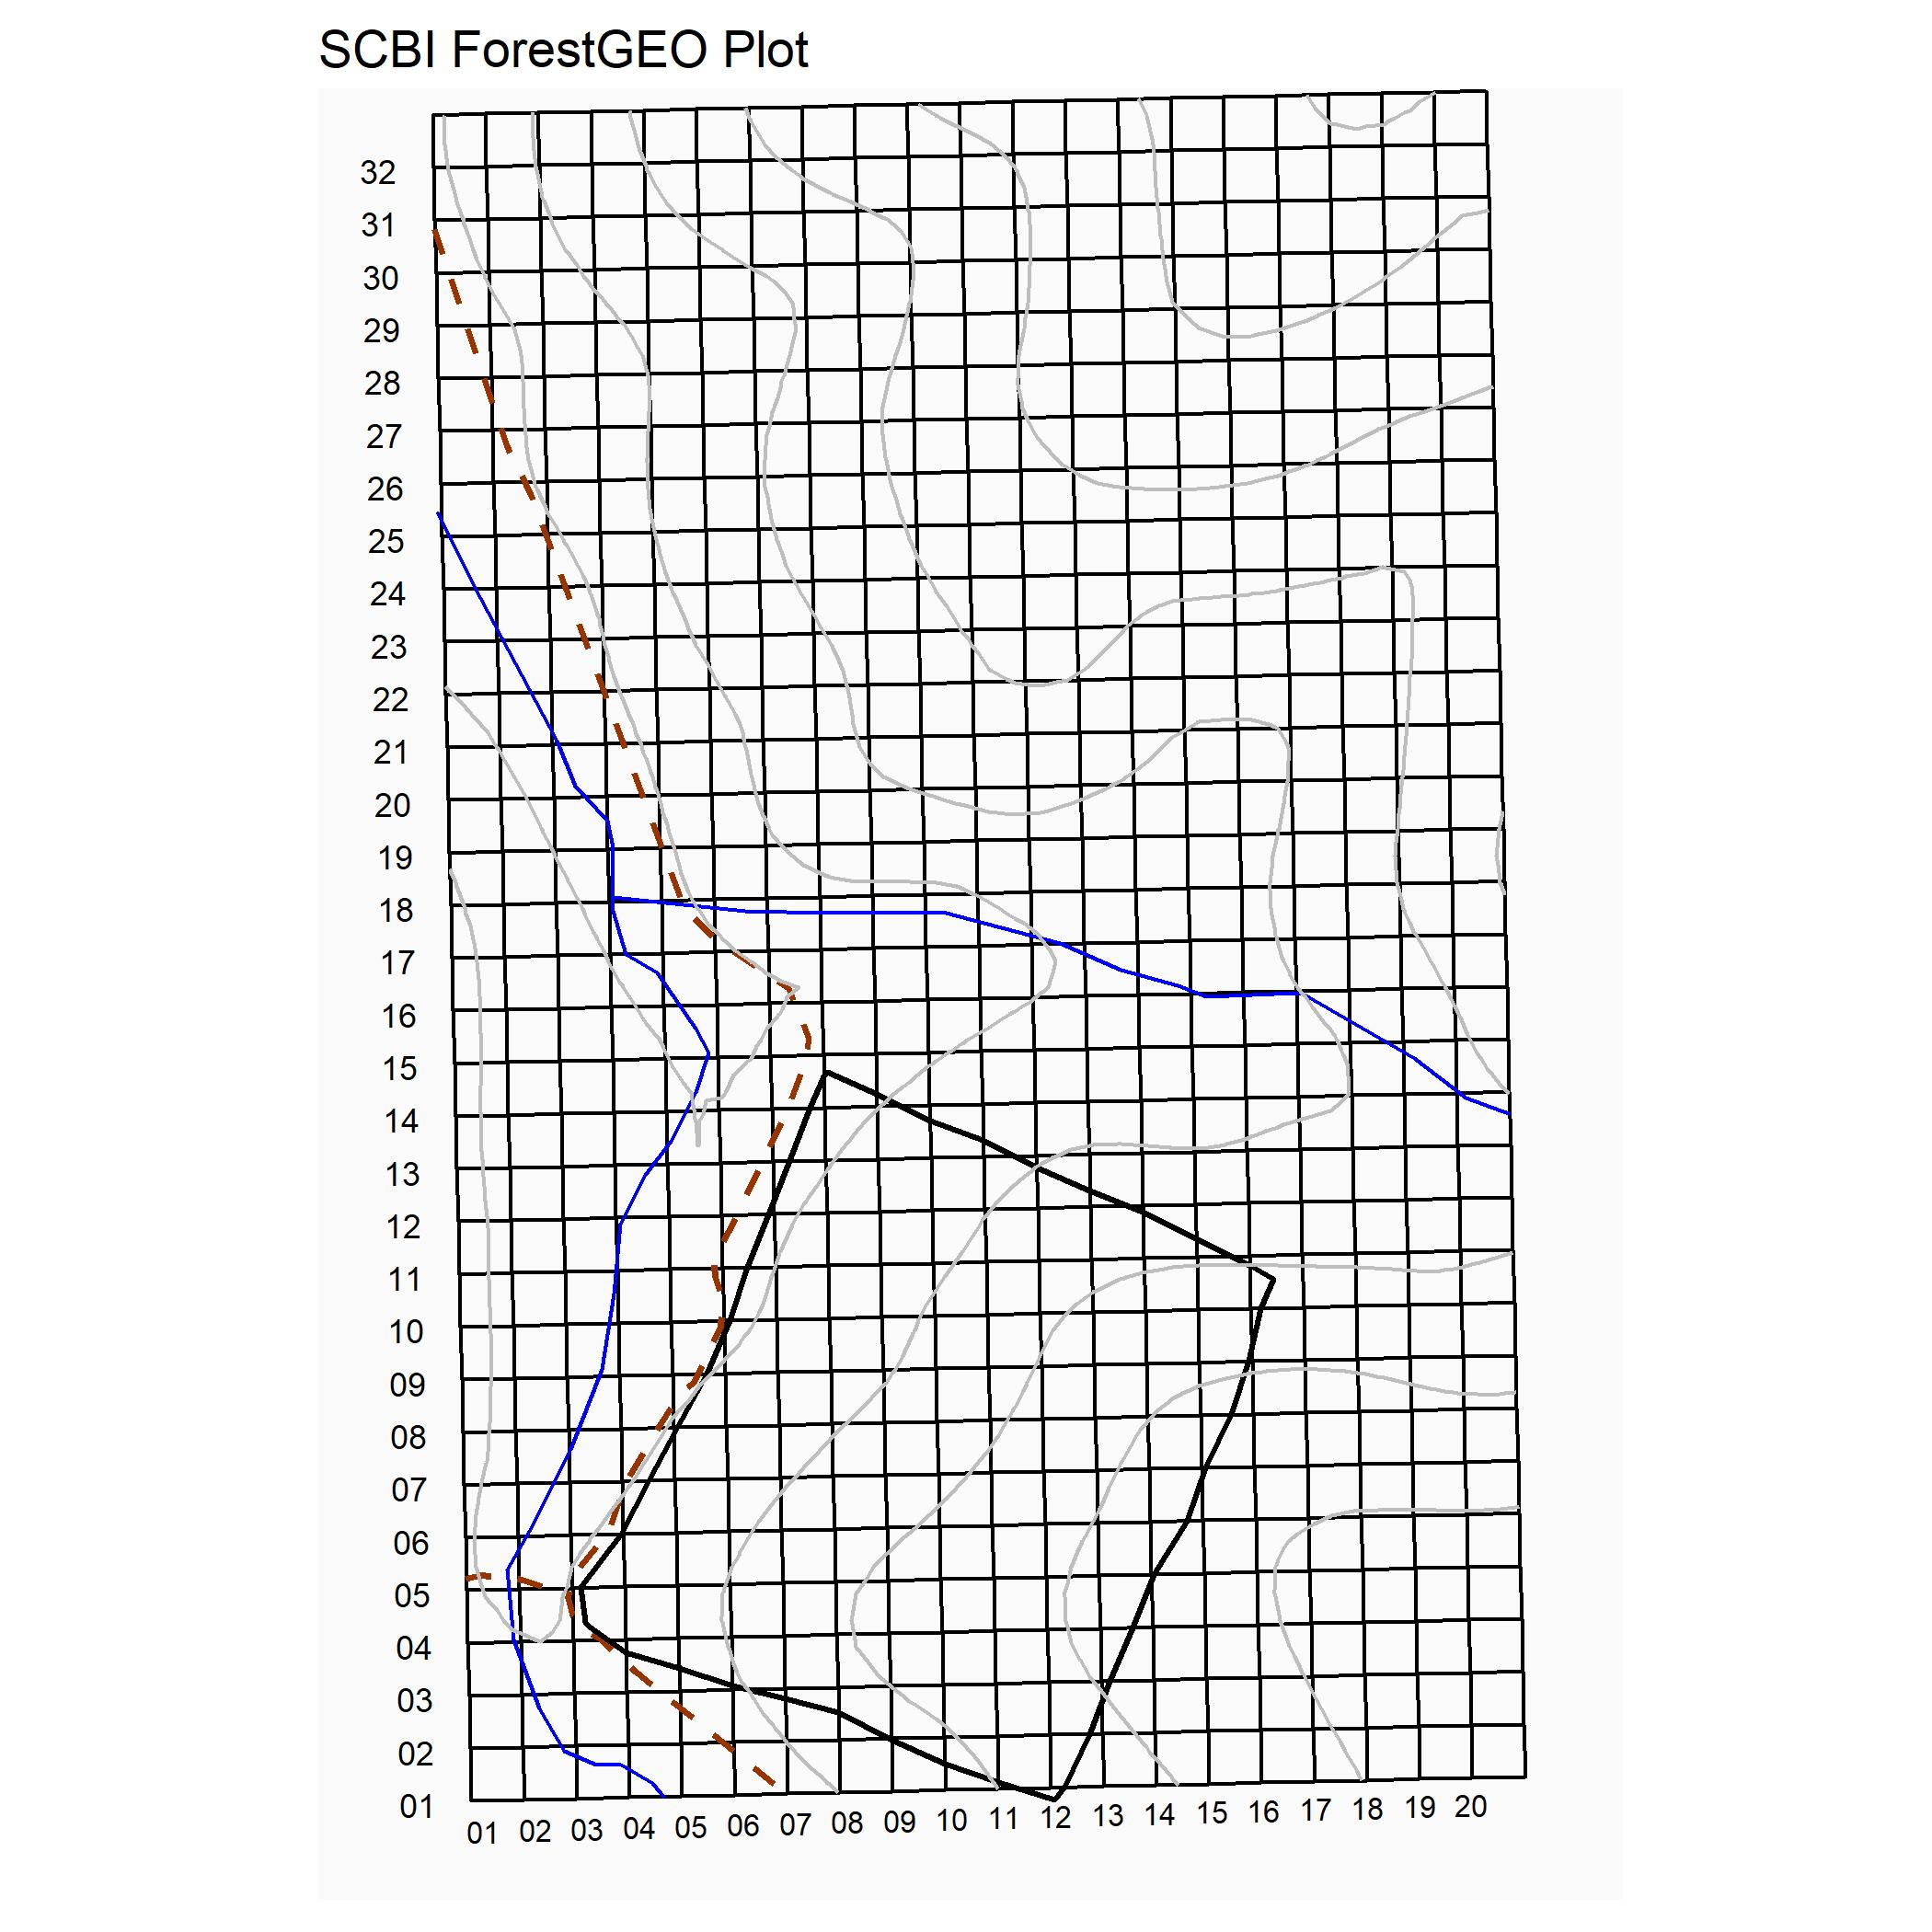
\includegraphics[width=1\linewidth]{tables_figures/ForestGEO_plot} \caption{Map of ForestGEO plot}\label{fig:unnamed-chunk-4}
\end{figure}

\emph{p50 and p80} We decided to include values of P50 and P80 in the
leaf traits model, defined by \citep{anderegg_meta-analysis_2016} as the
water potentials at which a species loses 50\% and 88\% {[}80\% by
proxy{]}, respectively, of hydraulic conductivity. Values were
calculated by (\textbf{insert new methods here??}), and were only
available for six species (\emph{C. glabra}, \emph{L. tulipifera},
\emph{Q. alba}, \emph{Q. prinus}, \emph{Q. rubra}, and \emph{Q.
velutina}). Because of this, the model runs were considered to be
incomplete due to the exclusion of the other 8 species. Results revealed
neither p50 nor p80 to be significant, thus for the full analysis we
decided to drop the two traits in order to include all species in the
full analysis.

(see Issue \#32)

\textbf{include TWI by trait graphs (2) here}

\bibliography{book.bib,packages.bib}


\end{document}
